\section{Testmiljø}
I dette afsnit præsenteres testmiljøet der sat op til at teste robottens færdigheder.

\subsection{Formål}
Formålet med et testmiljø er for bedre at kunne kontrollere omgivelserne.
Dette giver mindre unøjagtigheder ifht. hvis det skulle testes i et nyt miljø hver gang og man kan sammenligne resultater.

\subsection{Opsætning}
Testmiljøet er
Størrelse: 189*261

\begin{figure}
\begin{tikzpicture}
\node[anchor=south west,inner sep=0] at (0,0) {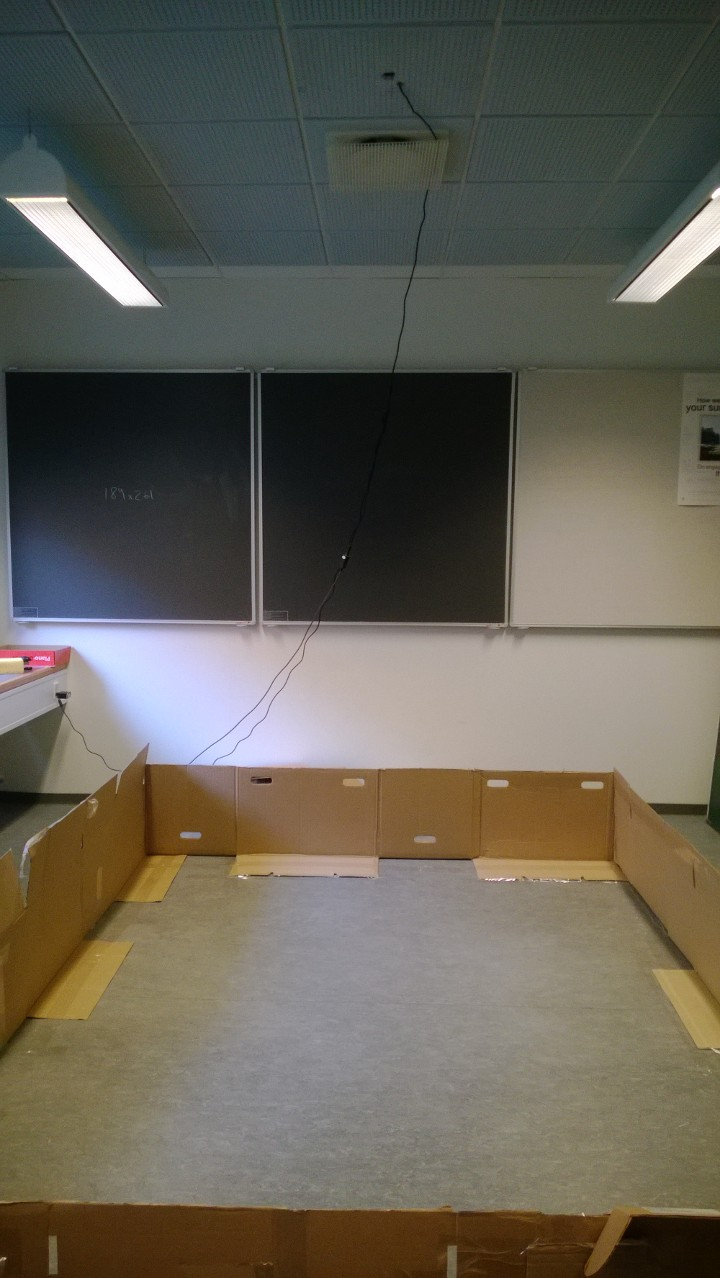
\includegraphics[width=\textwidth/2]{./verden/forfra}};
    \draw [->, red, ultra thick] (5.5,10.5) -- (4.2,11.2);
\end{tikzpicture}
\caption{Testmiljøet set forfra. Bemærk kinecten monteret i en loftplade(rød pil) med hul til RGB-kameraet.}
\label{testmiljo:forfra}
\end{figure}

\begin{figure}
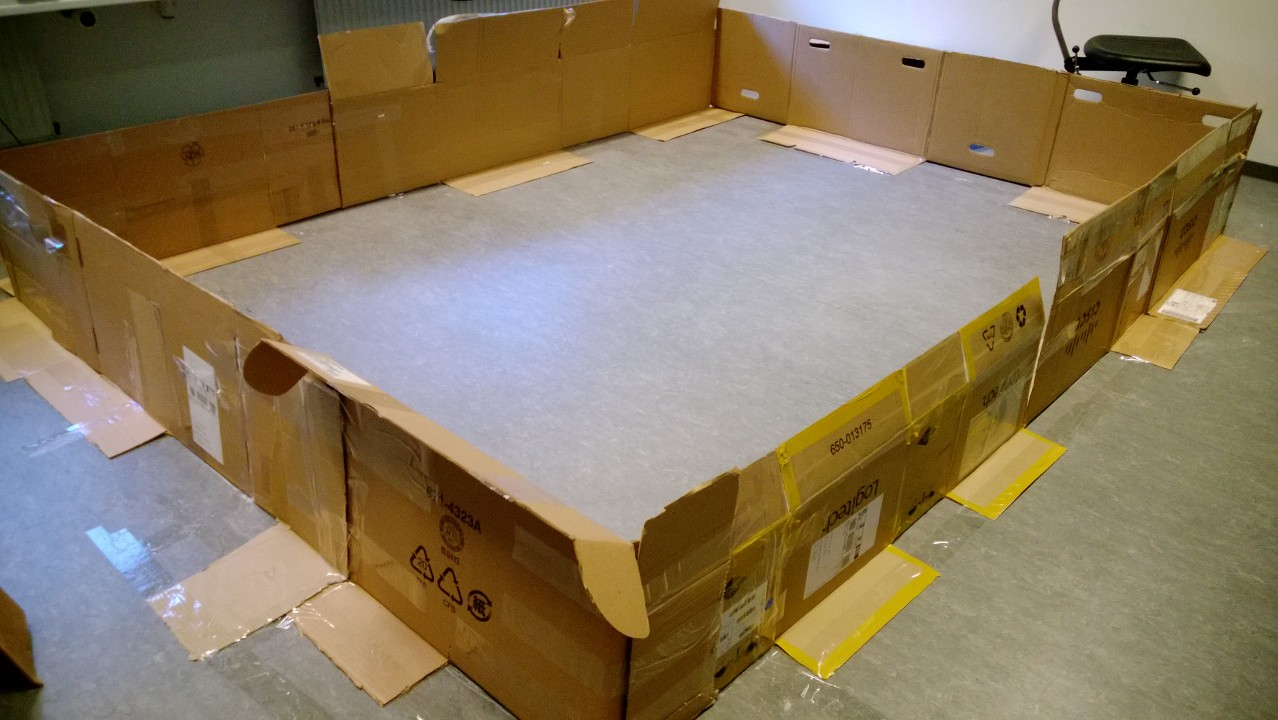
\includegraphics[width=\textwidth]{./verden/perspektiv}
\label{testmiljo:perspektiv}
\caption{Testmiljøet set i perspektiv.}
\end{figure}
\begin{figure}
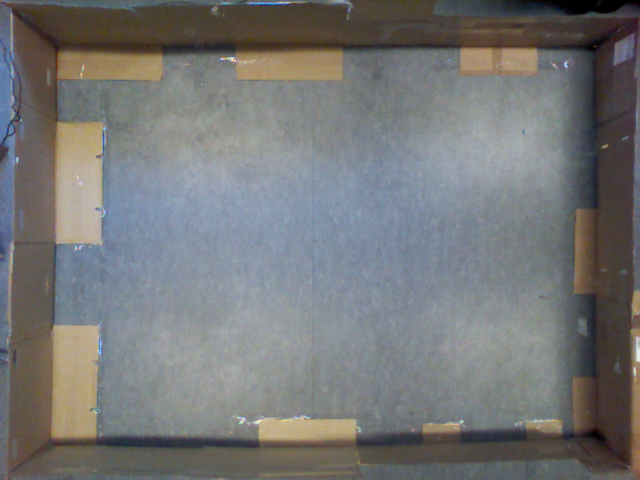
\includegraphics{./verden/oppefra}
\caption{Testmiljøet set fra kinecten.}
\label{testmiljo:oppefra}
\end{figure}